%!TEX root = ../main.tex

\chapter{Introduzione}
\label{chp:intro}
Questa tesi si pone l'obiettivo di trattare diversi ambiti del campo energetico: si parte con la definizione di fonte energetica cioè: \enquote{Una qualsiasi sostanza, materiale o fenomeno naturale o artificiale che può essere utilizzato per produrre energia}.
Partendo da questa si è effettuata una divisione per capire quali energie avessero una natura rinnovabile e quali invece non rinnovabile.
\begin{figure}[H]
    \centering
    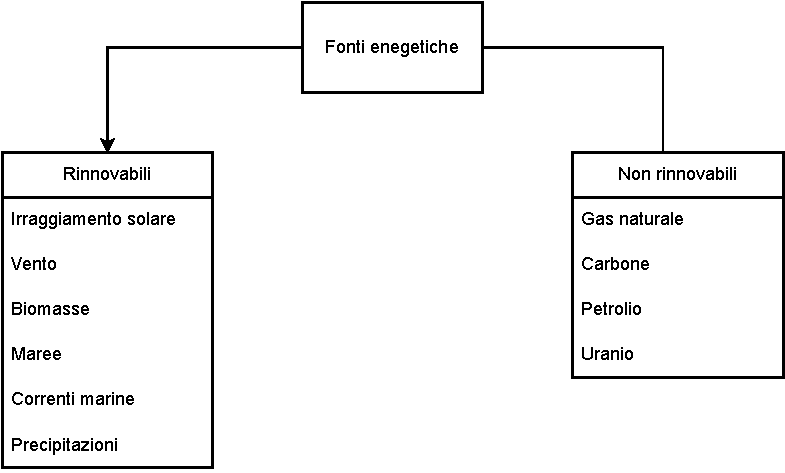
\includegraphics[height=0.4\textwidth]{res/cap 1/diagramma intro}
    \caption{Diagramma della prima suddivisione delle fonti energetiche}
\end{figure}\noindent
Si procede poi con una descrizione dettagliata prima delle fonti rinnovabili andando a definire la loro origine, le proprietà energetiche ed eventuali problematiche o accortezze che devono essere note per sfruttarle.\\
Si prosegue con una descrizione delle fonti partendo da quelle rinnovabili e descrivendo i fenomeni naturali che ne danno origine per poi procedere con la stesa metodologia con quelle non rinnovabili.\\
Il capitolo successivo tratterà gli impianti utilizzati per sfruttare le fonti precedentemente citate: in questo caso verranno trattati solo gli impianti rinnovabili in quanto di maggior interesse per quest'elaborato.
Per ciascun impianto saranno descritti i punti salienti che ne permettono l'applicazione, per ciascuna fonte potrebbero essere presenti più tipologie di impianti in tal caso saranno descritte singolarmente per metterne il luce le differenze.
\newpage
\begin{wrapfigure}{l}{5.5cm}
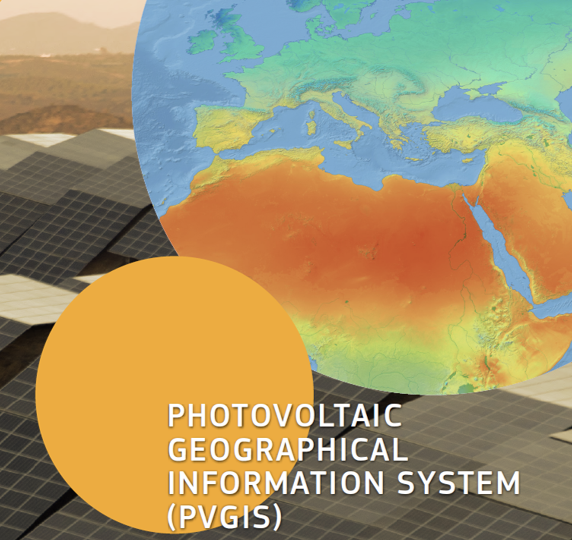
\includegraphics[width=5.5cm]{res/cap 1/PVGIS tool}
\end{wrapfigure} 
Per introdurre il caso studio che questa tesi si propone di illustrare, mi servirò di un tool offerto dal Joint Research Centre chiamato PVGIS: un capitolo ne tratterà l'accurata descrizione per trasmettere al lettore le potenzialità di tale strumento.
Questo, infatti, permette sia di effettuare in automatico calcoli sulla produzioni di diverse tipologie di impianti che di esportare dati grezzi da rielaborare poi con strumenti esterni.\\
Lo studio che condurrò come conclusione di questo elaborato sarà mirato a evidenziare le differenze costruttive che un impianto fotovoltaico riscontra in diverse locazioni geografiche e quanto le caratteristiche di esse, pur essendo alla stessa longitudine, ne influenzino la produzione.
\par
Le scelte delle collocazione degli impianti saranno effettuate cercando di evitare che il loro funzionamento sia alterato da condizioni meteo anomale per la regione o che siano influenzate dalla morfologia del territorio.